% This is a sample LaTeX input file.  (Version of 12 August 2004.)
%
% A '%' character causes TeX to ignore all remaining text on the line,
% and is used for comments like this one.

\documentclass{article}      % Specifies the document class

                            % The preamble begins here.
\title{Short Injector\\Quantum Cascade Laser Model}  % Declares the document's title.
\author{Kale J. Franz\\kfranz@princeton.edu}      % Declares the author's name.
\date{\today}      % Deleting this command produces today's date.

\usepackage{amsmath}
\usepackage{exscale}
\usepackage{graphicx}
%\usepackage{tex4ht}

\newcommand{\ip}[2]{(#1, #2)}
                             % Defines \ip{arg1}{arg2} to mean
                             % (arg1, arg2).

%\newcommand{\ip}[2]{\langle #1 | #2\rangle}
                             % This is an alternative definition of
                             % \ip that is commented out.

\addtolength{\voffset}{-1in}
\addtolength{\hoffset}{-1in}
\addtolength{\textwidth}{2in}
\addtolength{\textheight}{2in}
\addtolength{\marginparwidth}{-100pt}

\begin{document}             % End of preamble and beginning of text.

\maketitle                   % Produces the title.

\bigskip
\begin{center}
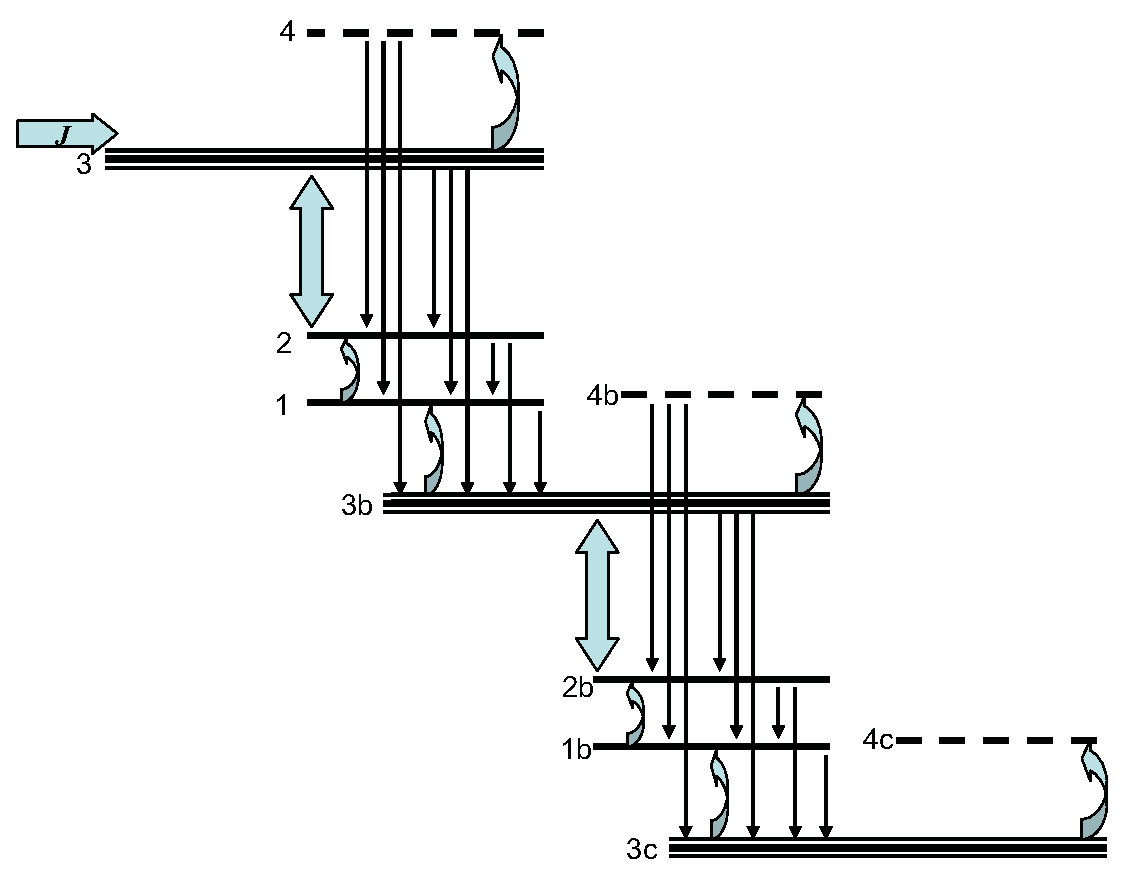
\includegraphics[width=7in]{diagram}
\end{center}
\bigskip

\begin{align}
\frac{dN_3}{dt} &= \frac{J}{q} - \frac{N_3}{\tau_{32}} - \frac{N_3}{\tau_{31}} - \frac{N_3}{\tau_{33b}} - \frac{N_3~e^{-\frac{E_{43}}{kT}}}{\tau_{4}} - \frac{N_3~e^{-\frac{E_{13b}}{kT}}}{\tau_{1}} - \frac{1}{N_p} \frac{c_0}{n_\mathit{eff}} g N_{ph} \nonumber\\
%
\frac{dN_2}{dt} &= \frac{N_4}{\tau_{42}} + \frac{N_3}{\tau_{32}} + \frac{N_{1}~e^{-\frac{E_{21}}{kT}}}{\tau_{2}} - \frac{N_2}{\tau_{21}} - \frac{N_2}{\tau_{23b}} + \frac{1}{N_p} \frac{c_0}{n_\mathit{eff}} g N_{ph} \nonumber\\
%
\frac{dN_1}{dt} &= \frac{N_4}{\tau_{41}} + \frac{N_3}{\tau_{31}} + \frac{N_2}{\tau_{21}} + \frac{(N_{3b}+n_{inj})e^{-\frac{E_{13b}}{kT}}}{\tau_{1}} - \frac{N_1}{\tau_{13b}} - \frac{N_{1}~e^{-\frac{E_{21}}{kT}}}{\tau_{2}}\nonumber\\
%
\frac{dN_4}{dt} &= \frac{(N_{3b}+n_{inj})e^{-\frac{E_{43b}}{kT}}}{\tau_{4}} - \frac{N_4}{\tau_{4}} \nonumber\\
%
\frac{dN_{3b}}{dt} &= \frac{N_4}{\tau_{43}} + \frac{N_4}{\tau_{43b}} + \frac{N_3}{\tau_{33b}} +\frac{N_2}{\tau_{23b}} + \frac{N_1}{\tau_{13b}} \nonumber\\
&~~~- \frac{N_3}{\tau_{32}} - \frac{N_3}{\tau_{31}} - \frac{N_3}{\tau_{33b}} - \frac{N_3~e^{-\frac{E_{43}}{kT}}}{\tau_{4}} - \frac{N_3~e^{-\frac{E_{13b}}{kT}}}{\tau_{1}} - \frac{1}{N_p} \frac{c_0}{n_\mathit{eff}} g N_{ph} \nonumber\\
%
\frac{dN_{ph}}{dt} &= \Gamma \frac{c_0}{n_\mathit{eff}} g N_{ph} - \frac{N_{ph}}{\tau_{ph}} \nonumber\\
%
g &= \frac{2 q^2 E_{32} z_{32}^2}{\hbar c_0 \epsilon_0 n_\mathit{eff} L_p~\delta E_{32}} (N_{3b}-N_2) \nonumber
\end{align}
\\
constants\\
$E_{32}$ = 254 meV\\
$E_{43}$ = 79\\
$E_{21}$ = 38\\
$E_{13b}$ = 74\\
\\
$z_{32}$ = 17 {\AA}\\
$L_p$ = 291 {\AA}\\
\\
$\tau_{43}$ = 0.954 ps\\
$\tau_{42}$ = 6.81\\
$\tau_{41}$ = 7.21\\
$\tau_{43b}$ = 5.42\\
\\
$\tau_{32}$ = 5.04\\
$\tau_{31}$ = 3.84\\
$\tau_{33b}$ = 8.26\\
\\
$\tau_{21}$ = 0.285\\
$\tau_{23b}$ = 1.27\\
\\
$\tau_{13b}$ = 0.291\\
\\
all $N_i$ have units of 1/area








\end{document}               % End of document.
\endinput 